\documentclass[../main.tex]{subfiles}
\begin{document}

\section{Linear models}
In this section we will going to analyze a linear model for classification and regression (Supervised Learning) both as task in function approximation. 

This is a \textbf{Parametric model}: A learning model that summarizes data with a set of parameters of fixed size (independent of the number of training examples) is called a parametric model.
\begin{itemize}
    \item \textbf{Given}: Training examples as $<input,output>=<x,d>$, we have labeled examples for some for some unknown function $f$. (For us $f$ is known only at the given example points).
    
    \item \textbf{Find}: a good approximation to $f$ (that can used for prediction on unseen data $\mathbf{x}'$
\end{itemize}

The target value \textbf{d} (or \textbf{t} or \textbf{y}), given by the teacher according to $f(\textbf{x})$, are numerical/ categorical label:
\begin{itemize}
    \item Classification: $f(x)$ return the (assumed) correct class for $x$, where $f(x)$ is a discrete valued function.
    
    \item Regression:  approximate a real-valued target function (in $\mathbb{R}$ o $\mathbb{R}^K$).
\end{itemize}

Here some Data notation in figure \ref{fig:data_notation}:
\begin{figure}[H]
    \centering
    \includegraphics[scale = 0.4]{lectures/2_linear_model/data_notation.png}
    \caption{Data notation for this section}
    \label{fig:data_notation}
\end{figure}

Now will we start to see linear models for Regression and classification where the H (hypothesis space is linear). Same model can be applied for both tasks and we will see how.

\begin{flushright}
\textit{"Despite the great inroads made by modern nonparametric regression techniques, linear models remain important, and so we need to understand them well."} (Hastie)
\end{flushright}

The linear model has been the mainstay of statistics and has a lot of studies and in many books (mathematics, statistics, numerical analysis, applicative fields, ML, ...). This model is also used/included in more complex models.

We will start with the simplest form: linear in the input variables.

\subsection{Regression}
Let's see first how we can formulate the learning problem as a \textbf{Least mean square (LMS)} problem and let's start to see it in a simplified setting: \textbf{univariate case}.

A regression task is the process of estimating of a real-value function on the basis of finite set of noisy samples, we have known pairs $(x, f(x) + \text{random noise})$ and we want to find an $h$ (hypothesis) that fit the data. See figure \ref{fig:linear_model_regression_exp}.
\begin{figure}
    \centering
    \includegraphics[scale = 0.6]{lectures/2_linear_model/regression_exp.png}
    \caption{Regression Example}
    \label{fig:linear_model_regression_exp}
\end{figure}

We want to solve it (how to find $\mathbf{w}$) in a systematic way.

\subsubsection{Univariate Linear Regression}

Univariate case, simple linear regression:
\begin{itemize}
    \item we start with 1 input variable $x$ and 1 output variable $y$
    
    \item we assume a model $h_w(x)$ expressed as:
    $$ h_w(x) = out = w_1x + w_0$$
    where $\mathbf{w}$ are real-valued \textbf{coefficients/free parameters (weights)}.
\end{itemize}

\begin{center}
    The idea is \textbf{fitting} the data by a  “straight line”.
\end{center}

In this case we have Infinite hypothesis space (continuous $w$ values) but we have nice solution from classical math (going back to Gauss/Legendre ~1795!).\\
Surprisingly we can “learn” by this basic tool and although simple it include many relevant concept of modern ML and it is
a basis of evolved methods in the field.

\noindent $\Rightarrow$ \textbf{Learning via LMS}:\\
\textbf{Learn}: means find the $\textbf{w}$ such that minimize error/empirical loss (bestdata fitting – on the training set with $l$ examples).

\begin{itemize}
    \item Given a set of $l$ training example $(x_p, y_p)$
    \item find $h_w(x)$ in the form: $w_1x + w_0$ (hence the values of $w$) that minimizes the expected loss on the training data.
\end{itemize}

As Loss function we will use the square of errors, Least (Mean) Square: find $w$ to minimize the residual sum of squares: $argmin_w \norm{Error(\mathbf{w})}$ 
\[\begin{aligned}
    Loss(h_\mathbf{w}) = E(\textbf{w}) &= \sum_{p = 1}^{l} (y_p - h_\mathbf{w}(x_p))^2 =\\
                            &=\sum_{p = 1}^{l} (y_p - (w_1x_p + w_0))^2
.\end{aligned}\]
Where $x_p$ is p-th input/patter/example, $y_p$ the output for $p$, $w$ free par., $l$ num. of examples.

\textbf{Note}: 
\begin{itemize}
    \item to have the mean, divide by l
    \item On the notation: Indeed for the univariate case, with 1 variable: $x_p = x_{p,l} = (x_p)_l$
\end{itemize}
The method of least squares is a standard approach to the approximate solution of over-determined systems, i.e., sets of equations in which there are more equations than unknowns.
\begin{figure}[H]
    \centering
    \includegraphics[scale = 0.5]{lectures/2_linear_model/learning_lms.png}
\end{figure}

\textbf{Note}: Why the mean square error with the $L_2$ norm? Because is a differentiable function that gives always positive values.

\noindent $\Rightarrow$ \textbf{How to solve?}:\\
Remember: local minimum as stationary point: the gradient is null:
$$ \frac{\partial E(\mathbf{w})}{\partial{w_i}} = 0 \; , \; i = 1, \dots,  \text{dim\_input}+1 = 1, \dots,  n+1$$
For the simple Lin. Regr. (2 free parameters):
$$ \frac{\partial E(\mathbf{w})}{\partial{w_i}} = 0 \qquad \qquad \frac{\partial E(\mathbf{w_0})}{\partial{w_1}} = 0 $$

\begin{figure}
    \centering
    \includegraphics[scale = 0.4]{lectures/2_linear_model/loss_gradient_2.png}
    \caption{Loss function plot with two free parameters}
    \label{fig:loss_gradient_2}
\end{figure}

We have a convex loss function, so there is no local minima and there is a closed form. The solution is:
\begin{figure}[H]
    \centering
    \includegraphics[scale = 0.4]{lectures/2_linear_model/solution_regression_two_par.png}
\end{figure}
It isn't mandatory to memorize this formula \textbf{but} for exercise try to reproduce the math to arrive there\ldots

Let's compute the gradient for 1 (each) patter p:

\begin{equation*}\label{eq:pareto mle2}
    \begin{aligned}
    \frac{\partial E(\mathbf{w})}{\partial{w_i}} = \frac{\partial(y-h_{\textbf{w}}(x))^2}{\partial{w_i}} =
    2(y-h_{\textbf{w}}(x))\frac{\partial(y-h_{\textbf{w}}(x))}{\partial{w_i}} =\\
    =2(y-h_{\textbf{w}(x)}))\frac{\partial(y-(w_1x+w_0))}{\partial{w_i}}
    \end{aligned}
\end{equation*}

and we will have:
\[
\frac{\partial E(\mathbf{w})}{\partial{w_0}} = -2(y - h_{\mathbf{w}}(x))  \qquad;\qquad \frac{\partial E(\mathbf{w})}{\partial{w_1}} = -2(y - h_{\mathbf{w}}(x))x
.\] 
then we will sum up for l patterns $(x_p,y_p)$:
\[
\frac{\partial E(\mathbf{w})}{\partial{w_0}} = -2\sum_{p = 1}^{l}(y_p - h_{\mathbf{w}}(x_p)) \qquad;\qquad \frac{\partial E(\mathbf{w})}{\partial{w_1}} = -2\sum_{p = 1}^{l}(y_p - h_{\mathbf{w}}(x_p))x_p
.\] 

\subsubsection{Linear Regression with multidimensional inputs case}
Assuming column vector $\mathbf{x},\, \mathbf{w} \in \mathbb{R}^n$, number of data $l$:
$$
\mathbf{w}^T\mathbf{x} + w_0 = w_0 +w_1 x_1 + w_2 x_2 + \dots + w_n x_n = w_0 + \sum_{i=1}^{n} w_i x_i
$$
Note:
\begin{itemize}
    \item that often (in NN), as before, the transpose notation T in $w^T$ is omitted
    \item $w_0$ is the intercept/threshold/bias/offset (has nothing to do with the inductive bias, bias is just a name here)
\end{itemize}

Often it is convenient to include the constant $x_0 = 1$ so that we can write:
$$ \mathbf{w}^T\mathbf{x} = \mathbf{x}^T\mathbf{w} \;,\; \mathbf{x}^T = [1, x_1, x_2, \dots, x_n] \;\text{and}\; \mathbf{w^T} = [w_0, w_1, w_2, \dots, w_n]$$

So, the “linear“ model is now: 
$$ h(\mathbf{x}_p) = \mathbf{x}_p\mathbf{w} = \sum_{i = 0}^{n} x_{p,i}w_i \;, \; \text{$w_i$ continuous (free) parameters “weights”}$$

\subsection{Classification}
We want now to use the same linear model (with LMS) presented for the regression task and use it for the classification task. The problem in Classification is shown in figure \ref{fig:2_classification_example_problem}

\begin{figure}[H]
    \centering
    \includegraphics[scale = 0.3]{lectures/2_linear_model/2_classification_example_problem.png}
    \caption{A classification problem (Data may be generated by gaussian distribution (for each class) with different means
or by a mixture of different low variance gaussian distributions)}
    \label{fig:2_classification_example_problem}
\end{figure}
We have 200 points generated in $\mathbb{R}^2$ from an unknown distribution, 100 in each of
two classes and we want to build a rule to predict the color of future points.

\noindent \textbf{We reuse the linear model for the classification task}:

The same models (used for regression) can be used for classification: categorical targets, e.g. $0/1$ or $-1/+1$

\begin{itemize}
    \item In this case we use an hyperplane ($\mathbf{wx}$) assuming negative or positive values.
    \item We exploit such models to decide if a point $\mathbf{x}$ belong to positive or negative zone of the hyperplane (to classify it)
    \item So we want to set $\mathbf{w}$ (by learning) s.t. we get good classification accuracy
\end{itemize}

\noindent \textbf{Geometrical view: hyperplane}:

We define an hyperplaen: $\mathbf{w}^T\mathbf{x}$, see figure \ref{fig:2_hyperplane} where our hyperplane is:
$$ \mathbf{w}^T\mathbf{x} = w_1x_1 + w_2x_2 +w_0 = 0$$
\begin{figure}[ht]
    \centering
    \includegraphics[scale = 0.6]{lectures/2_linear_model/2_hyperplane.png}
    \caption{Geometrical view: hyperplane}
    \label{fig:2_hyperplane}
\end{figure}


\noindent \textbf{Geometrical view: classifier}:\\
In this case our hypothesis ($h(x)$) is called \textbf{Linear threshold unit (LTU)} and is defined as follow:
\begin{figure}[H]
    \centering
    \includegraphics[scale = 0.4]{lectures/2_linear_model/2_LTU.png}
\end{figure}
In case of $w_0$ included in $\mathbf{w}$:
$$ h(\mathbf{x}_p) = sign(\mathbf{x}^T_p\mathbf{w}) = sign(\sum_{i = 0}^{n}x_{p,i}w_i)$$

\noindent A Geometrical view of our classifier is shown in figur \ref{fig:2_hyperplane_classifier}
\begin{figure}[ht]
    \centering
    \includegraphics[scale = 0.3]{lectures/2_linear_model/2_hyperplane_classifier.png}
    \caption{Geometrical view: hyperplane}
    \label{fig:2_hyperplane_classifier}
\end{figure}

\noindent \textbf{Classification by linear decision boundary}:\\
The classification may be viewed as the allocation of the input space in decision regions (e.g. 0/1) and the linear decision boundary can solve a linearly separable problem.

\begin{example}
    Linear separator on 2-dim instance space where our hypothesis space is composed by all the possible hyperplane (how the weight ($\mathbf{w}$) change).
$$\mathbf{x} = (x_1, x_2) \in \mathbb{R}^2 \;,\; f(x) = 0/1 \; \text{(or  -1/+1)}$$
\begin{figure}[H]
    \centering
    \includegraphics[scale = 0.3]{lectures/2_linear_model/2_linear_decision_boundary.png}
\end{figure}
\end{example}
In general the solution is not unique: there are many possible hyperplanes separating, let's see some hyperplane properties and how the hyperplane change with different $\mathbf{w}$ values.

\textbf{Hyperplane properties}:
\begin{figure}[H]
    \centering
    \includegraphics[scale = 0.3]{lectures/2_linear_model/2_hyperplane_prop.png}
\end{figure}
\begin{itemize}
    \item If $w_0=0$ the line goes through the origin of the coordinate system.
    \item If $n > 2 \;\; \rightarrow \;\;$ hyperplane 
    \item Scaling freedom: the same hyperplane multiplying $\mathbf{w}$ by K
    \item $\mathbf{w}$ is a vector orthogonal to the hyperplane, given $\mathbf{x_a}, \mathbf{x_b}$ (belonging to the hyperplane): $$\mathbf{x_a^Tw}+w_0=0 \;;\; \mathbf{x_a^Tw}+w_0=0 \rightarrow \mathbf{w^T}(\mathbf{x_a- x_b})=0 \rightarrow \text{orthogonal vectors}$$
    \item The best Hyperplane (the solution) is not unique.
\end{itemize}

\subsubsection{Role of Threshold $w_0$}%
Consider the bias $w_0$ in the LTU (Linear Threshold Unit). Asking for:
\[
    h(\v{x}) = \v{w}^T\v{x} + w_0 \ge 0
.\] 
Is the same that:
\[
    h(\v{x}) = \v{w}^T\v{x} \ge -w_0
.\] 
Wich $-w_0$ is now assumed as the "threshold" value.
\begin{itemize}
    \item The two form identify the same positive zone of the classifier.
    \item The second form emphatizes the role of the bias as threshold value to "activate" the $+1$ output of the classifier.
\end{itemize}

Here two examples:

\textbf{(AIMA) Classify a new data ($x_1,x_2$)}
\begin{figure}[H]
    \centering
    \includegraphics[scale = 0.6]{lectures/2_linear_model/2_example_clas_1.png}
\end{figure}

\textbf{Spam}
\begin{figure}[H]
    \centering
    \includegraphics[scale = 0.6]{lectures/2_linear_model/2_example_clas_2.png}
\end{figure}

\subsection{Learning Algorithms}
A learning algorithm is divided into two types:
\begin{itemize}
    \item \textbf{Eager}: Analyze the training data and construct an explicit hypothesis.
    \item \textbf{Lazy}: Store the training data and wait until a test data point is presented, then construct an ad hoc hypothesis to classify that one data point.
\end{itemize}
The linear model expected to construct an explict hypothesis from the training set, so the learning algorithm for the linear model is \textbf{Eager}.

We are going to introduce 2 \emph{learning algorithms} for the regression and for the classification task using a linear model, both based on \emph{LMS}.
\begin{itemize}
    \item A direct approach based on \textbf{normal equation} solution
    \item An iterative approach based on \textbf{gradient descent}
\end{itemize}
The learning algorithm has 


We start redefining the learning problem and the loss for them (for l data and multidimensional inputs).

\textbf{The learning problem (classification tasks)}\\
\textbf{Given} a set of $l$ training example $( \mathbf{x}_i, y_i)$ and a loss function (measure) $L$, we want to \textbf{find} the weight vector $\textbf{w}$ that minimizes the expected loss on the training data.

$$ R_{emp} = \frac{1}{l}\sum_{i = 1}^{l} L(h(\mathbf{x}_i),y_i) $$

For classification: Using a piecewise constant (over $sign(\mathbf{w^Tx})$ ) for the loss can make this a difficult problem because it is not continuous and differentiable. Assume we still use the least squares (as for the regression case).

\begin{figure}[H]
    \centering
    \includegraphics[scale = 0.3]{lectures/2_linear_model/2_loss_classification_smo.png}
    \caption{\scriptsize Example of Loss for the classifiation of a Positive instance. Both Loss satisfies the minimization of error.}
    \label{fig:2_loss_classification_smo}
\end{figure}
Initially, we can make the optimization problem easier by replacing the original objective function \textbf{L} by a smooth, differentiable function. For example, consider the mean squared error. See figure \ref{fig:2_loss_classification_smo}.

\noindent \textbf{Learning (a classifier) by Least Squares}:

\noindent\textbf{Given} a set of $l$ training example $( \mathbf{x}_i, y_i)$, \textbf{Find} optimal values for w (for fitting of Training data) by using the \textbf{least squares} that minimize the residual sum of squares:

$$ E(\mathbf{w}) = 1/l \sum_{i = 1}^{l} (y_i - \mathbf{x}_i^T\mathbf{w})^2 = \left\lVert\mathbf{y} - \mathbf{Xw} \right\rVert ^2$$

\begin{center}
    Min error: if $y_i=1$ then $x_i^Tw\rightarrow 1$ ; if $y_i=0$ then  $x_i^Tw\rightarrow 0$
\end{center} 

\textbf{Important}: In $E(\mathbf{W})$ we do not use $h(\mathbf{x})$, as for regression, but to hold a continuous differentiable loss (because $h(\mathbf{x})=sign(\mathbf{wx})$ for classification) we will use $\mathbf{x}_i^T\mathbf{w}$

This is a \emph{quadratic function} so the minimum always exists (but may be not unique).\\
($X$ is a matrix $\mathbf{l\, x\, n}$ with a row for each input vector $\mathbf{x}_i$).

\subsubsection{Normal equation and direct approach solution}
Differentiating $E(\mathbf{w})$ with respect to $\mathbf{w}$ we get the normal equation (point with gradient of E w.r.t $\mathbf{w} =0$):
$$ \mathbf{(X^TX)w = X^Ty}$$

\begin{proof} Now we want to compute $\frac{\partial E(\mathbf{w})}{\mathbf{w}_j} = 0 \;\; , \;\; j = 0, \dots, n$

$E(\mathbf{w}) = \sum_{i = 1}^{l}(y_i - \sum_{t = 0}^{n} w_t x_{i,t} )^2 =  \sum_{i = 1}^{l} (\delta_i(\mathbf{w}))^2 \;\;   \text{($l$ patterns)}$

$$\frac{\partial E(\mathbf{w})}{\mathbf{w}_j} = 2\sum_{i = 1}^{l} \delta_i(\mathbf{w}) \frac{\partial (\delta_i(\mathbf{w}))}{\partial \mathbf{w}_j} =   2\sum_{i = 1}^{l} \delta_i(\mathbf{w}) \frac{\partial (y_i - \sum_{t = 0}^{n} w_t x_{i,t} )}{\partial \mathbf{w}_j}=\quad  \quad$$
$$=2\sum_{i = 1}^{l} \delta_i(\mathbf{w}) (-x_{i,j}) = -2\sum_{i = 1}^{l} x_{i,j} \delta_i(\mathbf{w}) =
-2\sum_{i = 1}^{l} x_{i,j}(y_i - \sum_{t = 0}^{n} w_t x_{i,t} )  = 0
$$

$$\sum_{i = 1}^{l}x_{i,j}y_i = \sum_{i = 1}^{l}\sum_{t = 1}^{n} w_t x_{i,t} x_{i,j}  \;\; , \;\; j = 0, \dots, n$$

$$ \mathbf{X^Ty = (X^TX)w}$$
\end{proof}

So, if $ \mathbf{(X^TX)}$ is not singular the unique solution is given by:
$$ \mathbf{w = (X^TX)^{-1}X^Ty = X^+y} $$ 

Else the solution are infinite (satisfying the normal equation):
\begin{center}
    we can choose the min norm (w) solution.
\end{center}

\noindent\textbf{note}: ($\mathbf{X}^+$ is the Moore-Penrose pseudoinverse also if X is not invertible)

\noindent \textbf{Direct approach by SVD}:\\
The Singular Value Decomposition can be used for computing the pseudoinverse of a matrix:
\[
    \boldsymbol{X} = \boldsymbol{U}\boldsymbol{\Sigma}\boldsymbol{V}^T \implies  \boldsymbol{X}^+ = \boldsymbol{V}\boldsymbol{\Sigma}^+\boldsymbol{U}^T
.\] 
Where $\boldsymbol{\Sigma}$ are the diagonals values.

Moreover we can apply directly SVD to compute $ \mathbf{w =X^+y} $ obtaining the minimal norm (on w) solution of least squares problem.
\subsubsection{Gradient descent}
An iterative approach based on  \emph{gradient descent}:
Previous derivation suggest the line to construct an iterative algorithm based on :
$$\frac{\partial E(\mathbf{w})}{\partial\mathbf{w}_j} = -2\sum_{i = 1}^{l} (y_i - \mathbf{x}_i^T\mathbf{w})(\mathbf{x}_i)_j
= 
-\sum_{i=1}^{l} 2\delta_i x_{i, j}
$$
Where
\begin{itemize}
    \item $\mathbf{x}_i$: i-th input pattern
    \item $y_i$: the output for $p$
    \item $\mathbf{w}$: free parameters
    \item $l$: numbers of examples
    \item $(\mathbf{x}_i)_j$: component $j$ of pattern $i$
\end{itemize}
Gradient (ascent direction): we can move toward the minimum with a gradient descent (- gradient of $E(\mathbf{w})$).

\textbf{Local search}: begins with initial weight vector. Modifies it iteratively to decrease up to minimize the error function (steepest descent).
\begin{figure}[H]
  \centering
  \subfloat[Gradient descent]{\includegraphics[width=0.5\textwidth]{lectures/2_linear_model/gradient_1.png}\label{fig:2_linear_model_gradient_1}}
  \hfill
  \subfloat[H for 2 –w linear model]{\includegraphics[width=0.5\textwidth]{lectures/2_linear_model/2_model_gradient_2_w}\label{fig:2_linear_model_H_for_2_w}}
  \caption{\scriptsize In the left we can see that choosing the direction $-\frac{\partial E(\v{w}) }{\partial \v{w}} $ we are moving to the minimum of $E(\v{w})$ (step by step).}
\end{figure}

\noindent\textbf{Delta Rule}\\
A training rule whose key idea behind the delta rule is to use gradient descent to search the hypothesis space of possible weight vectors to find the weights that best fit the training examples.\\
The «movements» will be made iteratively according to the \textbf{Learning Rule}:
$$\mathbf{w}_{new} = \mathbf{w}_{old} + eta \cdot \Delta \mathbf{w}$$
where $eta$ is the step size, $0<eta<1$ or a value. $\Delta \mathbf{w}$ is $-\frac{\partial E(\v{w}) }{\partial \v{w}}$ (vectorial).

\textbf{learning rate ($\eta$) - eta} =: speed/stability trade-off and is the step size: can be (gradually) decreased to zero (guarantee convergence, avoiding oscillation around the min.): many variants will be introduced later.

In figure \ref{fig:2_learning_rate} is shown how the gradient descent change with different learning rate and figure \ref{fig:2_learning_curve} is shown how the learning curve can change.

\begin{figure}[H]
    \centering
    \includegraphics[scale = 0.29]{lectures/2_linear_model/2_learning_rate.png}
    \caption{Different learning rate bring to different convergences speed and also different results.}
    \label{fig:2_learning_rate}
\end{figure}
\noindent\textbf{Gradient descent algorithm}
\begin{figure}[H]
    \centering
    \includegraphics[scale = 0.5]{lectures/2_linear_model/Gradient_alg.png}
    \label{fig:2_gradient_alg}
\end{figure}

In the stardard case we use $\Delta \v{w}/ l$ : least mean squares (when you divide by l). It's good to normalize the value of the graident, otherwise could be too large and could lead to oscillations (bad learning curve).

There are two versions of the algorithm:
\begin{itemize}
    \item For \textbf{batch version} the gradient is the sum over all the $l$ patterns (using $p$):
$$\frac{\partial E(\mathbf{w})}{\partial\mathbf{w}_i} = -2\sum_{p = 1}^{l} (y_p - \mathbf{x}_p^T\mathbf{w})x_{p,i}$$

So, to calculate the gradient of the cost function, we need to sum the cost of each pattern. If we have 3 million patterns, we have to loop through 3 million times or use the dot product.\\
\noindent Note that:
\begin{itemize}
    \item $x_{p,i}$ is the component $i$ of pattern $p$
    \item $2$ is constant that can be ignored to develop the algorithm
    \item we typically use \emph{LMS} (use $1/l$ in front of the sum)
    \item provide a more “precise” evaluation of the gradient over a set of $l$ data
    \item We upgrade the weights after this sum
\end{itemize}

\item For the \textbf{on-line/stochastic version} we upgrade the weights with the error that is computed for each pattern.
$$\frac{\partial E_p(\mathbf{w})}{\partial\mathbf{w}_i} = -2(y_p - \mathbf{x}_p^T\mathbf{w})x_{p,i}$$
In SGD weights are updated upon examining each training example so, we only use 1 example for each learning step. Because it’s using only one example at a time, its path to the minima more random than that of the batch gradient. Usually, before for-looping, you need to randomly shuffle the training examples.
\item We will see intermediate cases later (as \textbf{mini-batch}): Mini-batch gradient descent uses n data points (instead of 1 sample in SGD) at each iteration.
\end{itemize}
Here an example showing how the trajectory change with different gradient descent algorithm:
\begin{figure}[H]
    \centering
    \includegraphics[scale = 0.3]{lectures/2_linear_model/gradient_versions.png}
    \caption{Gradient descent variants trajectory towards minimum}
    \label{fig:2_gradient_trajectory}
\end{figure}

\noindent \textbf{Learning curve examples}: the curve can change with different gradient algorithm and different value of the learning rate:
\begin{figure}[H]
    \centering
    \includegraphics[scale = 0.4]{lectures/2_linear_model/2_learning_curve.png}
    \caption{Learning curve examples}
    \label{fig:2_learning_curve}
\end{figure}
\subsubsection*{Gradient descent as Error correction rule}
\[\begin{aligned}
&\Delta w_j = \sum_{p = 1}^{l} (y_p - \mathbf{x}_p^T\mathbf{w})(\mathbf{x}_p)_j\\
&\v{w}_{new} = \v{w} + \eta \cdot \Delta \v{w}
.\end{aligned}\]
This is an “error correction” rule (Widrow-Hoff) that change the $w$ proportionally to the error (target-output):

For example:
\begin{itemize}
    \item $(target - output) = err=0 \rightarrow$ no correction
    
    \item $(input_j>0)\,\, if\,\,err\,\,+ \;\; (\text{output is too low}):$
    $$increase\,\, w_j \rightarrow\,\, increase\,\, output \rightarrow less\,\, err$$
    
    \item $(input_j>0)\,\, if\,\,err\,\,-\;\;(\text{output is too high}): $
    $$decrease\,\, w_j \rightarrow\,\, reduce\,\, output \rightarrow less\,\, err$$

    \item $(input_j<0)\,\, if\,\,err\,\,+\;\;(\text{output is too low}): $
    $$decrease\,\, w_j \rightarrow\,\, increase\,\, output \rightarrow less\,\, err$$  

    \item $(input_j<0)\,\, if\,\,err\,\,- \;\; (\text{output is too high}):$
    $$increase\,\, w_j \rightarrow\,\, reduce\,\, output \rightarrow less\,\, err$$
\end{itemize}
It allow us to search through an \emph{infinite hypothesis} space and it can be easily always applied for \emph{continues $H$} and differentiable loss.

\textbf{NOTE}: Is the gradient descent efficient? Many improvement are possible: Newton and quasi-newton methods, Conjugate Gradient, ...

Here and example of Delta-W as Error Correction Learning rule:
\begin{figure}[H]
    \centering
    \includegraphics[scale = 0.4]{lectures/2_linear_model/2_e_g_correction_rule.png}
\end{figure}

\subsubsection{Summarizing}
\begin{itemize}
    \item Model trained (on tr set) with LS (LMS) on $\mathbf{wx}$ by the simple gradient descent algorithm used for linear regression
    
    \item Model used for classification applying the threshold function $h(\mathbf{x}) = sign(\mathbf{wx})$
    
    \item The error can be computed as classification error or number of misclassified patterns (not only by the Mean Square Error)
    \begin{figure}[H]
        \centering
        \includegraphics[scale = 0.4]{lectures/2_linear_model/2_summarizing.png}
    \end{figure}

    \item ACCURACY = mean of correctly classified = $(l-num\_err)/l$
\end{itemize}

\newpage

\subsection{Linear model on a classification problem}
Let's analyze the problem shown in figure \ref{fig:2_classification_example_problem_2} problem and let's apply the linear model on the training data set.
\begin{figure}[H]
  \centering
  \subfloat[Raw data]{\includegraphics[width=0.45\textwidth]{lectures/2_linear_model/2_classification_example_problem.png}\label{fig:2_classification_example_problem_2}}
  \hfill
  \subfloat[After LMS algorithm]{\includegraphics[width=0.45\textwidth]{lectures/2_linear_model/2_classification_example_problem_with_lm.png}\label{fig:2_classification_example_problem_lm_2}}
  \caption{Solution of a classification example with LMS}
\end{figure}
A classification example in two dimensions. The classes are coded as a binary variable.
In figure \ref{fig:2_classification_example_problem_lm_2} we can see the result of the linear model: The line is the decision boundary defined by $\mathbf{x^Tw} = 0.5$.

\[
    h(\textbf{x}) = \left\{
                \begin{array}{ll}
                  1 \quad if \;\; \mathbf{x^Tw}>0.5\\
                  0 \quad otherwise
                \end{array}
              \right.
\]

The decision boundary is $\{\mathbf{x} \;|\; \mathbf{x^Tw} = 0.5 \}$ is linear (and seems to make many errors on the training data). Is it true?

\noindent \textbf{Good or bad approximation}:
Possible scenarios (we know the true target function!):
\begin{itemize}
    \item Scenario 1: The data in each class are generated from a Gaussian distribution with uncorrelated components, same variances, and different means.\\
    In this case $\Rightarrow$ the linear regression rule (by LS) is almost optimal (is the best one can do). The region of overlap is inevitable (due to errors in the input data). 
    \item Scenario 2: The data in each class are generated from a mixture of 10 gaussians in each class.\\
     In this case  $\Rightarrow$ the linear model is far too rigid: next models for it!
\end{itemize}

\subsection{Linear Model in ML: inductive bias (Mitchell style)}%
\begin{itemize}
    \item Language bias: the H is a set of linear functions (may be very restrictive and rigid)
    \item  Search bias: ordered search guided by the Least Squares minimization goal
	\begin{itemize}
	    \item For instance we could prefer a different method to obtain a restriction on the values of parameters, achieving a different solutions with other properties…
	    \item It shows that even for a “simple” model there are many possibilities.  We still need a principled approach! (see theory of ML)…
	\end{itemize}
\end{itemize}

\subsection{Linear regression (in statistics)}
In statistics, \textbf{linear regression} is used for two things:
\begin{itemize}
    \item to construct a simple formula that will predict a value or values for a variable
given the value of another variable.
    \item to test whether and how a given variable is related to another variable or variables.
\end{itemize}
Statistical Parametric models: note that, in general,"\textbf{linear}" does not refer to this straight line, but rather to the way in which the regression coefficients occur in the regression equation. (See next for “linear basis expansion”).

\noindent\textbf{NOTE}: Least squares corresponds to the maximum likelihood criterion if the
experimental errors have a normal distribution.

\subsection{Linear model (in ML): Inductive Bias (alla Mitchell)}
In the Linear model we have two Bias:
\begin{itemize}
    \item \textbf{Language bias}: the H is a set of linear functions (may be very restrictive and rigid)

    \item \textbf{Search bias}: ordered search guided by the Least Squares minimization goal: for instance we could prefer a different method to obtain a restriction on the values of parameters, achieving a different solutions with other properties...

\end{itemize}

It show that even for a “simple” model there are many possibilities. We still need a principled approach! (see theory of ML)...

\subsection{Limitations}
This linear model has some limitation: It's a \textbf{rigid model}.

\noindent$\blacksquare$ \textbf{Regression tasks for non linear problems}

\begin{minipage}{0.5\textwidth}
In this case we have a very poor solution, a linear model can't fit a non linear problem! we have to find a solution for it!
\end{minipage}
\hfill
\begin{minipage}{0.5\textwidth}
\includegraphics[width=\linewidth]{lectures/1_Introduction/intro_poly_1}
\end{minipage}
\newpage

\noindent$\blacksquare$\textbf{Classification tasks}
\begin{itemize}
    \item In geometry, two set of points in a two-dimensional plot are \textbf{linearly separable} when the two sets of points can be completely separated by a single line.
    \item In general, two groups are linearly separable in $n-dimensional$ space if they can be separated by an $(n-1)-dimensional$ hyperplane.
    \item The linear decision boundary can provide exact solutions only for linearly separable sets of points.
    \begin{figure}[H]
        \centering
        \includegraphics[scale = 0.2]{lectures/2_linear_model/2_linear_classifier_divide_right.png}
    \end{figure}
\end{itemize}

\textbf{Example: Conjunctions}\\
We can represent conjunctions by the linear models:
\begin{figure}[H]
    \centering
    \includegraphics[scale = 0.4]{lectures/2_linear_model/2_eg_conjunctions.png}
\end{figure}

\textbf{Example: 3 point}\\
Given 3 points, we can find a separation plane only if they are not aligned, otherwise no (3 aligned points with 0 in the middle and others 1):

\begin{figure}[H]
    \centering
    \includegraphics[scale = 0.4]{lectures/2_linear_model/2_eg_three_point.png}
\end{figure}

\textbf{Example: 4 points}\\
Given 4 points we can't always find a separtion plane (we can find a labeling such that the linear classifier fails to be perfect), e.g xor:
\begin{figure}[H]
    \centering
    \includegraphics[scale = 0.4]{lectures/2_linear_model/2_eg_xor.png}
\end{figure}


\subsection{A generalization}
The linear model is a very rigid model, here we will show a basis expansion. This allow to get more \textbf{Flexibility}.

\noindent$\blacksquare$\textbf{Regression task}\\
Basis transformation(\textbf{linear basis expansion}) :
$$h_w(\mathbf{x})=\sum_{k = 0}^{K} w_k\phi_k(\mathbf{x})$$
Augment the input vector with additional variables ($K>n$) which are transformations of $\mathbf{x}$ according to a function $\phi_k: R^n\rightarrow R$. $\phi$ can be every function.

E.g:
\begin{itemize}
    \item Polynomial representation of $x$: $\phi(x) = x_j^2$ or $\phi(x) = x_jx_i,$ or other functions
    \item Non-linear transformation of single inputs: $\phi(x) = log(x_j)$, $\phi(x) = root(x_j)$, ...
    \item Non-linear transformation of multiple input: $\phi(x) = \norm{x}$
    \item Splines, ...
\end{itemize}

This generalization is called: \textbf{dictionary} approaches and the model is linear in the parameters (also in phi, not in x!), so we can use the same learning algorithm as before!

\textbf{Example}:
\begin{itemize}
    \item 1-dim $x$ : $\phi_j(x) = x^j$ ($1-dim$ polynomial regression ($K=M$)):
    $$ h(\mathbf{x}) = w_0 + w_1x + w_2x^2 + \dots + w_Mx^M = \sum_{j = 0}^M w_jx^j$$
    
    \item any other, $\phi(\mathbf{x}) = \phi([x_1, x_2, x_3])$:
    $$  h(\mathbf{x}) = w_1x_1 + w_2x_2 + w_3 log(x_2)+ w_4 log(x_3) + w_5(x_2x_3) + w_0 $$
\end{itemize}

For \emph{classification task} we add sign before the sum.
\begin{itemize}
    \item \textbf{PROS}: Can model more complicated relationships (than linear). It is more expressive with more flexibility.
    \item \textbf{CONS}: With \emph{large} basis of functions, we easily risk \emph{overfitting}, hence we require methods for \emph{controlling the complexity} of the model. Furthermore:
    \begin{itemize}
        \item Phi are fixed before observing training data, it's hard to decide which $\phi$ will be good for our data! (versus adaptive /non-linear in parameters e.g. in Neural Network)
        \item \textit{Curse of dimensionality} (the volume of the problem space increases so fast that the available data become sparse).
    \end{itemize}
\end{itemize}

\subsection{Improvements}
\subsubsection{How to control model complexity? Regularization}
\noindent$\blacksquare$\textbf{Ridge regression (Tikhonov regularization)}\\
smoothed model $\rightarrow$ e.g. lower variance
\begin{figure}[H]
    \centering
    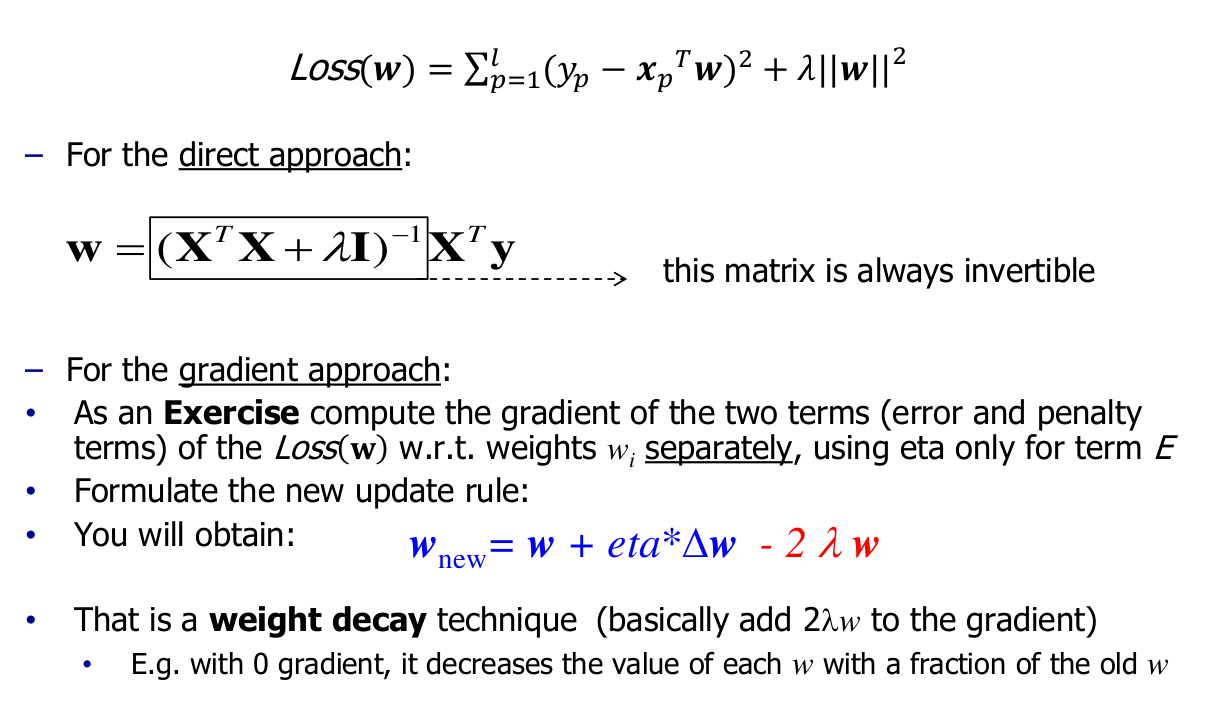
\includegraphics[scale = 0.3]{lectures/2_linear_model/tikhonov.png}
    \caption{Figura sbagliata\ldots}
    \label{fig:2_tikhonov}
\end{figure}
\textbf{Note}: For the objective function we use here the name Loss (used for the model training cost function) to distinguish from the Error E (useful to evaluate the model error and used for the data term inside this Loss).\\
Hence, differently from previous assumptions the two terms are not more equivalent in our use (in the course).

\textbf{Lambda ($\lambda$) regularization parameter}: 
$$ 0\leq \lambda < 1$$
Possible to add constraints to the sum of value of $\abs{w_j}$ favouring "sparse" models e.g. with less terms due to weights $w_j=0$ (i.e. less complex solutions): ridge regression [or lasso, et al. (by different norms)]

\begin{itemize}
    \item The penalty term \emph{penalizes high value of the weights} and tends to drive all the weights to smaller values (some weights values can go even to zero).
    \item It \emph{implements} a control of the model complexity
    \item This leads to a model with \emph{less VC-Dim}.
    \item $\lambda$ values can rule the underfitting/overfitting cases.
\end{itemize}
Tikhonov regularization can be applied for every function and allow us to control the VC-dim. It's better to have a big H space and then control the search bias with $\lambda$.

\textbf{Remember}: Can be applied to any kind of function, in this way you easily understand wich model is the simplest (just with one more parameter $\lambda$). This move the complexity to the \textbf{Search Bias} instead of \textbf{Language Bias}!

\newpage
\noindent$\blacksquare$\textbf{Example of control of model complexity:}\\
Let's suppose to have a regression task and we will use this $h(\mathbf{x})$:

$$ h(\mathbf{x}) = w_0 + w_1x + w_2x^2 + \dots + w_Mx^M = \sum_{j = 0}^M w_jx^j$$

$$ x : \phi_j(x) = x^j \text{($1-dim$ polynomial regression ($M = 9$))}$$
Let's see how we can control the complexity of the model:
\begin{itemize}
    \item in figure \ref{fig:2_lambda_1} we can see the case where $\lambda = 0$ and there is no regularization. In this case how $h(\mathbf{x})$ is in overfitting and the error $E(w) = 0$ on the training set. This model is too complex and is able to fit the noise too. (we have to control the complexity of the model in this case
    
    \item in figure \ref{fig:2_lambda_2} we use a small positive lambda ($\lambda = 0.0000000152$. The model has been regularized it and the VC-dim has been reduced too. This model seems to works much better.
    
    \item in figure \ref{fig:2_lambda_3} we use a very high lambda, close to 1 ($ln\lambda = 0$) and the model goes in underfitting.
\end{itemize}

From the three previous cases we understand that we need a trade-off and we need to find the right lamda value that does not make us go underfitting or overfitting.

\begin{figure}[ht]
  \centering
  \subfloat[Lambda = 0]{\includegraphics[width=0.5\textwidth]{{lectures/2_linear_model/lambda_1.png}}\label{fig:2_lambda_1}}
  \vskip\baselineskip
  \subfloat[$ln\lambda = -18$: lambda small positive]{\includegraphics[width=0.5\textwidth]{{lectures/2_linear_model/lambda_2.png}}\label{fig:2_lambda_2}}
  \hfill
  \subfloat[$ln\lambda = 0$: very high lambda, close to $1$]{\includegraphics[width=0.5\textwidth]{{lectures/2_linear_model/lambda_3.png}}\label{fig:2_lambda_3}}  
  \caption{9th Order Polynomial with control of complexity}
\end{figure}


\begin{figure}[H]
    \centering
    \includegraphics[scale = 0.5]{lectures/2_linear_model/lambda_0.png}
    \caption{Regularization: $E_{RMS}$ vs $ln\lambda$}
    \label{fig:2_lambda_0}
\end{figure}

In figure \ref{fig:2_lambda_0} we can see how the $E_{RMS}$ change with different value of $\lambda$ and figure \ref{fig:2_poly_coeff_with_reg} shows how the value of weights change with different value of $\lambda$.

\begin{figure}[H]
    \centering
    \includegraphics[scale = 0.3]{lectures/2_linear_model/2_polynomial_coefficients.png}
    \caption{Polynomial Coefficients}
    \label{fig:2_poly_coeff_with_reg}
\end{figure}


\subsubsection{Other Regularization Technology for Linear Models}
There is other technology used for regularization that we will introduce in later sections:
\begin{itemize}
    \item Ridge regression ($\norm{\cdot}_2$)
    \item Lasso ($\norm{\cdot}_1$)
    \item Elastic nets (use both $\norm{\cdot}_1$ and $\norm{\cdot}_2$)
\end{itemize}

The L2 norm penalizes the square value of the weight and tends to drive all the weights to smaller values. On the other hand, the L1 norm penalizes the absolute value of the weight and tends to drive some weights to exactly zero (while allowing some weights to be large) $\rightarrow$ toward feature selection!

\textbf{NOTE}: Unfortunately $\norm{\cdot}_1$ (absolute value) introduce a non differentiable so the loss needs other approaches.

\subsubsection{Others Improvements}
\begin{itemize}
    \item Inputs with added noise (data augmentation)
    \item Derived inputs: a small number of new variables is used in place of the x inputs, which are a linear combination of x.
    \begin{itemize}
        \item \textit{Principal Component Regression}
        \item \textit{Partial Least Squares}
    \end{itemize}
\end{itemize}

\subsection{Multi-class task}
There is two very simple approaches for multi-class:

\begin{itemize}
    \item \textbf{OVA (one-vs-all)}: a discriminant function for each class, built on top of real-valued binary classifiers:
    \begin{itemize}
        \item train K different binary classifiers, each one trained to distinguish the examples in a single class from the examples in all remaining classes.
        \item to classify a new example, the K classifiers are run, and the classifier which outputs the largest (most positive) value is chosen.
    \end{itemize}
        $$ h(\mathbf{x}) = \mbox{arg}\max_{i}h_i(\mathbf{x})$$ 

    e.g. Class 1-of-K rep: {red, green, blue} $\rightarrow$ (0,0,1), (0,1,0), (1,0,0). $\rightarrow$ solve 3 linear models.
    
    \item \textbf{AVA (all-vs-all = one-versus-one)}:
    Each classifier separates a pair of classes. Build $K(K-1)$ classifiers K-way multiclass problem, one classifier to distinguish each pair of classes $i$ and $j$.
    \begin{itemize}
        \item to classify a new example, all the classifiers are run, and the winner is the one with the
                max sum of outputs versus all the other classes OR the class with most votes
        $$ h(\mathbf{x}) = \mbox{arg}\;\max_{i} \; (\sum_{j}^{} h_{ij}(\mathbf{x}))$$ 
        \item training data set for each classifier is much smaller
    \end{itemize}
    
\end{itemize}
OVA, AVA suffers from ambiguities in that some regions of its input space may receive the same number of votes.

\noindent \textbf{Criticism}:
The problem can become not easy
\begin{figure}[H]
    \centering
    \includegraphics[scale = 0.35]{lectures/2_linear_model/2_multiclass_crit.png}
\end{figure}

\begin{itemize}
    \item Masking: classes can be masked by others (for high K) 
    \item A wide array of more sophisticated approaches for
multiclass classification exists ...
    \item Some models can deal directly with multi-output
\end{itemize}

\subsection{Other learner models for classification}
\begin{itemize}
    \item Linear Discriminant Analysis (also multi-class)
    \item Logistic regression\\
    $P(y | \mathbf{x})$  starting from modeling the class density as a know density
\end{itemize}

\begin{figure}[H]
    \centering
    \includegraphics[scale = 0.5]{lectures/2_linear_model/3_slide_end1.png}
\end{figure}
\begin{figure}[H]
    \centering
    \includegraphics[scale = 0.5]{lectures/2_linear_model/3_slide_end2.png}
\end{figure}
\end{document}


